\begin{verbatim}
%% To submit your paper:
\documentclass[draft,linenumbers]{AGUJournal}
\draftfalse

%% For final version.
% \documentclass{AGUJournal}

\journalname{Water Resource Research}

\begin{document}
\end{verbatim}

\begin{verbatim}
\title{A hierarchical model of daily stream temperature for regional predictions}

 \authors{Daniel J. Hocking\affil{1}\thanks{Current address, Department of Biology, Frostburg State University, Frostburg, MD, USA.},
 Benjamin H. Letcher\affil{1}, and Kyle O'Neil\affil{1}}

\affiliation{1}{US Geological Survey, Leetown Science Center, Conte Anadromous Fish Research Center, Turners Falls, MA, USA.}

\correspondingauthor{D. J. Hocking}{djhocking@frostburg.edu}
\end{verbatim}

\begin{verbatim}
%  List up to three key points (at least one is required)
%  Key Points summarize the main points and conclusions of the article
%  Each must be 100 characters or less with no special characters or punctuation 
\end{verbatim}

\begin{verbatim}
\begin{keypoints}
\item Flexible appraoch to modeling daily stream temperature across broad space
\item Allows for inclusion of short observed stream temperature time series
\item Air temperature effects influenced by precipitation and drainage area
\end{keypoints}
\end{verbatim}

\section{Abstract}\label{abstract}

Stream temperature is an important exogenous factor influence
populations of stream organisms such as fish, amphibians, and
invertebrates. Given the interest in maintaining cold water fisheries,
many states regulate stream protections based on temperature. Therefore,
having good models of stream temperature is important, particularly for
understanding thermal regimes in unsampled space and time. To help meet
this need, we developed a hierarchical model of daily stream temperature
and applied it to data from across the eastern United States. Our model
accomodates many of the key challenges associated with daily stream
temperature models including the non-linear relationship between air and
water at very low and very high temperatures, the lagged response of
water temperature to changes in air temperature, incomplete and widely
varying observed time series, spatial and temporal autocorrelation, and
the inclusion of predictors other than air temperature. We used xxxx
stream temperature records from xxxx streams to fit our model and xxxx
records witheld for model validation. Our model had a root mean squared
error of xxx for the fitted data and xxxx for the validation data,
indicating excellent fit and good predictive power. We then used our
model to predict daily stream temperatures from 1980 - 2015 for all
streams \textless{}200 \(km^2\) from Maine to Virginia. From these, we
calculated derived stream metrics including mean July temperature, mean
summer temperature, number of years where the maximum daily stream
temperature exceeded 20 C, and the thermal sensitivity of each stream
reach to changes in air temperature. Although generally water
temperature follows similar latitudinal and altitudinal patterns as air
temperature, there are considerable differences at local scales based on
moderating landscape and land-use factors. We made these metrics
available through the ecosheds.org web application so that managers and
policy makers can use this information in natural resource decision
making.

\section{Introduction}\label{introduction}

Temperature is a critical factor in regulating the physical, chemical,
and biological properties of streams. Warming stream temperatures
decrease dissolved oxygen, decrease water density, and alter the
circulation and stratification patterns of streams (refs).
Biogeochemical processes such as nitrogen and carbon cycling are also
temperature dependent and affect primary production, decomposition, and
eutrophication (refs). Both physical properties and biogeochemical
processes influence the suitability for organisms living in and using
the stream habitat beyond just primary producers. Additionally,
temperature can have direct effects on the biota, especially
poikliotherms such as invertebrates, amphibians, and fish {[}\emph{Xu et
al.}, 2010b, 2010a; \emph{Al-Chokhachy et al.}, 2013; e.g., \emph{Kanno
et al.}, 2013{]}. Given commercial and recreational interests, there is
a large body of literature describing the effects of temperature on
fish, particularly the negative effects of warming temperatures on
cool-water fishes such as salmonids . Finally, stream temperature can
even affect electricity, drinking water, and recreation (see van Vliet
et al 2011). Therefore, understanding and predicting stream temperatures
are important for a multitude of stakeholders.

Stream temperature models can be used for explanatory purposes
(understanding factors and mechanisms affecting temperature) and for
prediction. Predictions can be spatial and temporal including
forecasting and hindcasting. Predictions across space are especially
valuable because there is often a need for information at locations with
little or no observed temperature data. For example, many states have
regulations related to the management of streams classified as cold,
cool, and warm waters (refs), but because of the tremendous number of
headwater streams it is impossible classify most streams based on
observed data. Therefore, modeled stream temperature is needed to
classify most streams for regulatory purposes. Forecasting can provide
immediate information such as the expected temperature the next hour,
day, or week as well as long-term information about expected
temperatures months, years, and decades in the future. Hindcasting can
be used to examine temperature variability and trends over time and for
model validation. Both forecasting and hindcasting are useful for
understanding climate change effects on stream temperature regimes.

Given the importance of temperature in aquatic systems, it is not
surprising that there are a variety of models and approaches to
understanding and predicting stream temperature. Stream temperature
models are generally divided into three categories: deterministic (also
called process-based or mechanistic), stochastic, and statistical
{[}\emph{Caissie}, 2006; \emph{Benyahya et al.}, 2007; \emph{Chang and
Psaris}, 2013{]}. Deterministic models are based on heat transfer and
are often modeled using energy budgets {[}\emph{Caissie}, 2006;
\emph{Benyahya et al.}, 2007{]}. The models require large amounts of
detailed information on the physical properties of the stream and
adjacent landscape as well as hydrology and meteorology. These models
are useful for detailed re assessments and scenario testing. However,
the data requirements preclude the models from being applied over large
spatial extents.

Stochastic models attempt to combine pattern (seasonal and spatial
trends) with the random deviations to describe and predict environmental
data {[}\emph{Kiraly and Janosi}, 2002; \emph{Sura et al.}, 2006;
\emph{Chang and Psaris}, 2013{]}. Stochastic models of stream
temperature generally rely on relationships between air and water
temperature then with random noise and an autoregressive correlation,
often decomposed by seasonal and annual components. These models are
mostly commonly used to model daily temperature fluctuations because of
their ability to address autocorrelation and approximate the near-random
variability in environmental data {[}\emph{Caissie et al.}, 2001;
\emph{Kiraly and Janosi}, 2002; \emph{Ahmadi-Nedushan et al.}, 2007{]}.
A limitation is that the physical processes driving temperature
fluctuations are not elucidated with these models. They are generally
used to describe characteristics and patterns in a system and to
forecast these patterns in the future {[}\emph{Kiraly and Janosi},
2002{]}. Additionally, stochastic models rely on continuous, often long,
time series from a single or a few locations. Inference cannot be made
to other locations without assuming that the patterns and random
deviations are identical at those locations.

As with stochastic models, statistical models generally rely on
correlative relationships between air and water temperatures, but also
typically include a variety of other predictor variables such as basin,
landscape, and land-use characteristics. Statistical models are often
linear with normally distributed error and therefore used at weekly or
monthly time steps to avoid problems with temporal autocorrelation at
shorter time steps (e.g.~daily, hourly, sub-hourly). Parametric,
nonlinear regression models have been developed to provide more
information regarding mechanisms than traditional statistical models
without the detail of physical deterministic models {[}\emph{Mohseni et
al.}, 1998{]}. Researchers have also developed geospatial regression
models that account for spatial autocorrelation within dendritic stream
networks {[}\emph{Isaak et al.}, 2010; \emph{Peterson et al.}, 2010,
2013{]}. However, due to the complexity of the covariance structure of
network geostatistical models, they are best used for modeling single
temperature values across space (e.g.~summer maximum, July mean, etc.)
rather than daily temperatures {[}\emph{Peterson et al.}, 2007, 2010;
\emph{{Ver Hoef} and Peterson}, 2010{]}. Additionally, statistical
machine learning techniques such as artificial neural networks have been
used to model stream temperatures when unclear interactions,
nonlinearities, and spatial relationships are of particular concern
{[}\emph{Sivri et al.}, 2007, 2009; \emph{DeWeber and Wagner}, 2014b{]}.

In contrast with deterministic approaches, statistical models require
less detailed site-level data and therefore can be applied over greater
spatial extents than process-based models. They also can describe the
relationships between additional covariates and stream temperature,
which is a limitation of stochastic models. These relationships can be
used to understand and predict anthropogenic effects on stream
temperature such as timber harvest, impervious development, and water
control and release {[}\emph{Webb et al.}, 2008{]}. Quantifying the
relationship between anthropogenic effects, landscape characteristics,
meteorological patterns, and stream temperature allows for prediction to
new sites and times using statistical models. This is advantageous for
forecasting and hindcasting to predict and understand climate change
effects on stream temperatures. This is critical because not all streams
respond identically to air temperature changes and the idiosyncratic
responses may be predicted based interactions of known factors such as
flow, precipitation, forest cover, basin topology, impervious surfaces,
soil characteristics, geology, and impoundments {[}\emph{Webb et al.},
2008{]}.

Letcher et al. {[}{\textbf{???}}{]} outline six general challenges of
statistical stream temperature models including accounting for 1) the
non-linear relationship between air and water temperature at high and
low air temperatures, 2) different relationships between air and water
temperature in the spring and fall (hysteresis), 3) thermal inertia
resulting in lagged responses of water temperature to changes in air
temperature, 4) incomplete time series data and locations with large
differences in the amount of available data, 5) spatial and temporal
autocorrelation, and 6) important predictors of stream water temperature
other than air temperature. They developed a statistical model that
addresses aspects of non-linear relationships, hysteresis, thermal
inertia, and spatial and temporal autocorrelation but their analysis was
limited to a single small network of streams with long time series
{[}{\textbf{???}}{]}.

We describe a novel statistical model of daily stream temperature that
incorporates features of stochastic models and extends the Letcher et
al. {[}{\textbf{???}}{]} framework to large geographic areas. This model
handles time series data of widely varying duration from many sites
using a hierarchical mixed model approach to account for autocorrelation
at specific locations within watersheds. It incorporates catchment,
landscape, and meteorological covariates for explanatory and predictive
purposes. It includes an autoregressive function to account for temporal
autocorrelation in the time series, a challenge with other statistical
models at fine temporal resolution. Additionally, our hierarchical
Bayesian approach readily allows for complete accounting of uncertainty.
We use the model to predict daily stream temperature across the
northeastern United States over a 36-year time record.

\section{Methods}\label{methods}

\subsubsection{Water temperature data}\label{water-temperature-data}

We gathered stream temperature data from state and federal agencies,
individual academic researchers, and non-governmental organizations
(NGOs) from Maine to Virginia (Figure 1; Table 1?). The data were
collected using automated temperature loggers. The temporal frequency of
recording ranged from every 5 minutes to once per hour. This data was
consolidated in a PostgreSQL database linked to a web service at
\url{http://www.db.ecosheds.org}. Data collectors can upload data at
this website and choose whether to make the data publicly available or
not. The raw data is stored in the database and users can flag problem
values and time series. Only user-reviewed data are used in the analysis
and flagged values are excluded. For our analysis, we performed some
additional automated and visual quality assurance and quality control
(QAQC) on the sub-daily values, summarized to mean daily temperatures
and performed additional QAQC on the daily values. The QAQC was intended
to flag and remove values associated with logger malfunctions,
out-of-water events (including first and last days when loggers were
recording but not yet in streams), and days with incomplete data which
would alter the daily mean. The QAQC webtool used for flagging
questionable data can be found at \url{http://db.ecosheds.org/qaqc} We
also developed an R (ref) package for analyzing stream temperature data
from our database, including the QAQC functions which can be found at
\url{https://github.com/Conte-Ecology/conteStreamTemperature}. The R
scripts using these functions for our analysis are available at
\url{https://github.com/Conte-Ecology/conteStreamTemperature_northeast}.

\begin{figure}[htbp]
\centering
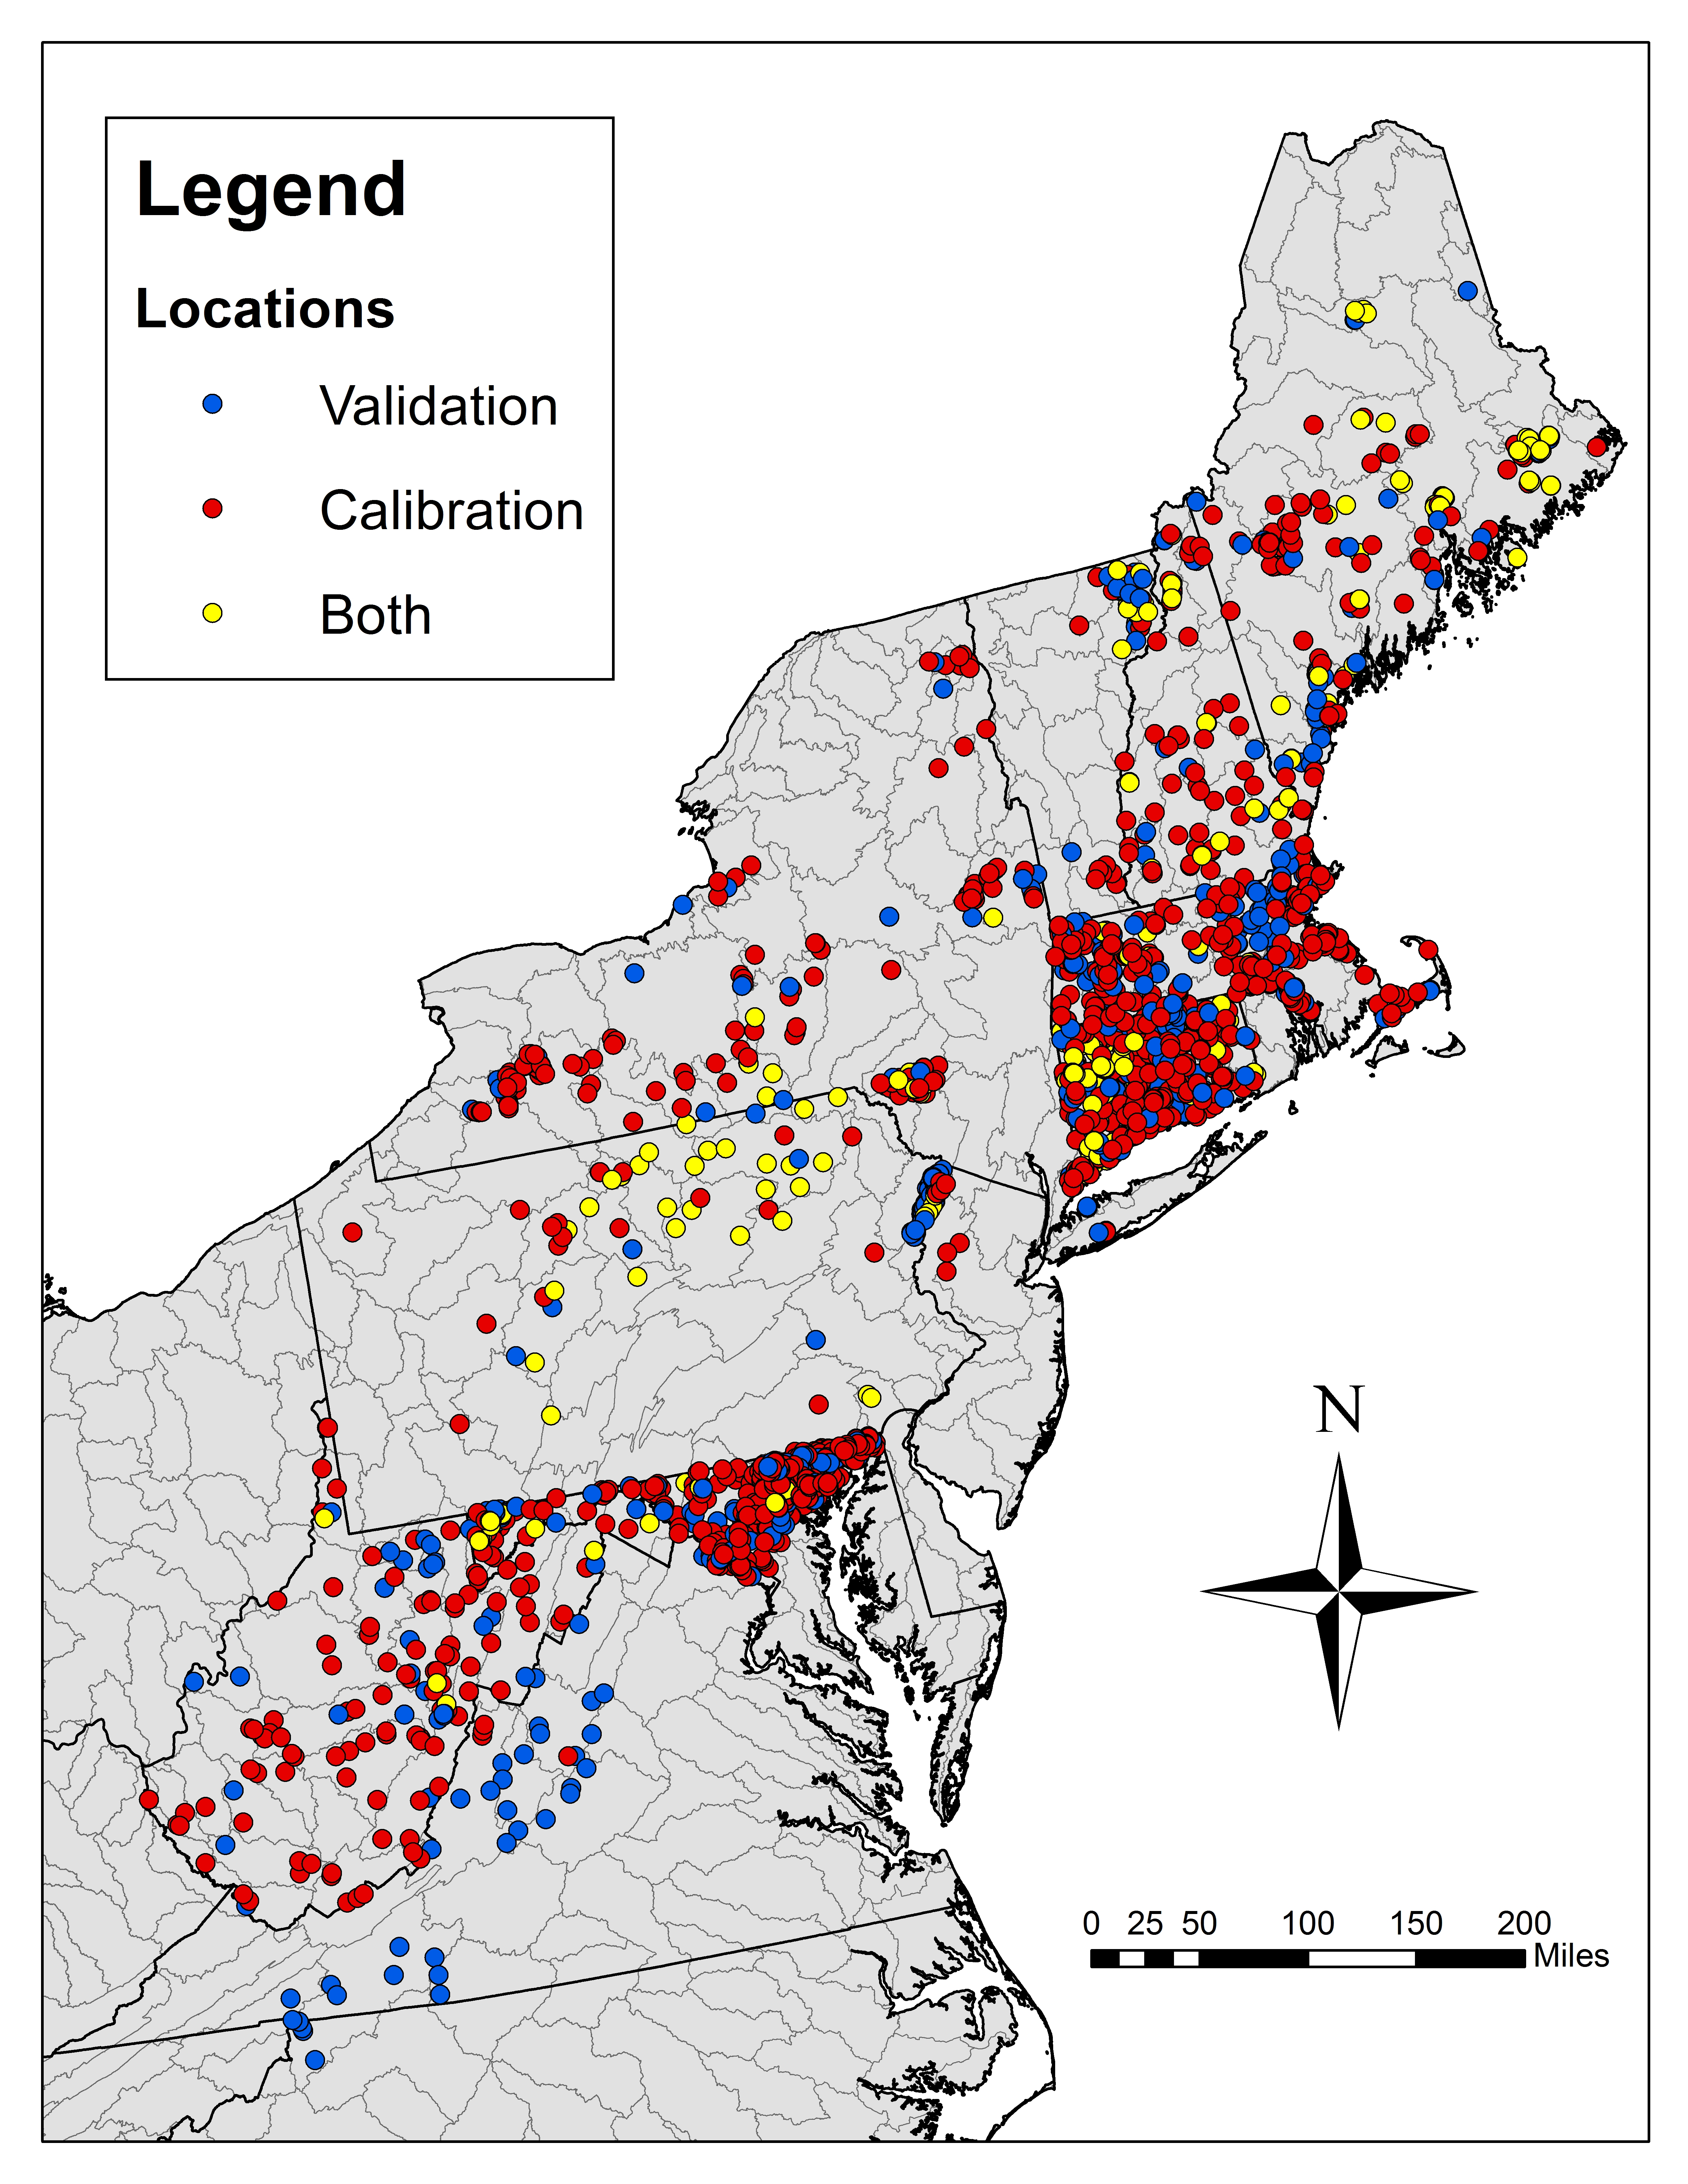
\includegraphics{Figures/Locations_Map.png}
\caption{Map of the sampling locations including data used in model
fitting (calibration), withheld for validation, and used in both fitting
and validation. Locations used in both fitting and validation indicate
that some years of data were used for one purpose and some for another,
no day-location combination was used in both fitting and validation. See
text for description of how validation data were chosen.}
\end{figure}

Stream reach (stream section between any two confluences) was our finest
spatial resolution for the analysis. In the rare case where we had
multiple logger locations within the same reach (2,894 locations from
2,413 reaches) recording at the same time, we used the mean value from
the loggers for a given day (Table 1). In the future, with sufficient
within reach data, it would be possible to use our modeling framework to
also estimate variability within reach by adding one more level to the
hierarchical structure of the model (see Statistical Model description
below).

Table 1. Summary of data used to model daily stream temperature. The
number of records represents the number of raw temperature measurements
(sub-daily) and locations used to create the daily water temperature
timeseries for \(N_{years}\) at 2,413 stream reaches (catchments).

\begin{longtable}[c]{@{}rrrrr@{}}
\toprule
State & \(N_{records}\) & \(N_{years}\) & \(N_{locations}\) &
\(N_{reaches}\)\tabularnewline
\midrule
\endhead
CT & 5,007,479 & 19 & 515 & 418\tabularnewline
DE & 294,591 & 10 & 1 & 1\tabularnewline
MA & 3,212,204 & 20 & 628 & 546\tabularnewline
MD & 258,076 & 13 & 497 & 402\tabularnewline
ME & 5,522,845 & 22 & 274 & 189\tabularnewline
NH & 17,191,459 & 9 & 151 & 124\tabularnewline
NJ & 247,974 & 4 & 61 & 42\tabularnewline
NY & 6,357,709 & 20 & 292 & 266\tabularnewline
PA & 17,280,353 & 10 & 162 & 142\tabularnewline
RI & 2,615 & 3 & 4 & 4\tabularnewline
VA & 159,334 & 2 & 41 & 41\tabularnewline
VT & 21,161 & 13 & 54 & 53\tabularnewline
WV & 835,882 & 8 & 214 & 185\tabularnewline
Totals: & 56,391,682 & 22 & 2894 & 2413\tabularnewline
\bottomrule
\end{longtable}

\subsubsection{Stream network
delineation}\label{stream-network-delineation}

Temperature logger locations were spatially mapped to the stream reaches
of a high resolution network of hydrologic catchments developed across
the Northeastern United States. The National Hydrography Dataset High
Resolution Delineation Version 2 (NHDHRDV2) maintains a higher
resolution and catchment areal consistency than the established NHDPlus
Version 2 dataset. The main purpose of the higher resolution was to
capture small headwaters that may be critical to ecological assessment.
A summary of this dataset with links to detailed documentation can be
found in the \href{http://conte-ecology.github.io/shedsGISData/}{SHEDS
Data project}.

\subsubsection{Meteorological and landscape
data}\label{meteorological-and-landscape-data}

The landscape and meteorological data were assembled from various
sources. These variables were spatially attributed to the hydrologic
catchments for incorporation into the model and include total drainage
area, percent riparian forest cover, daily precipitation, daily air
temperature, upstream impounded area, percent agriculture, and percent
high-intensity development. Further descriptions and data sources for
each of these variables are described in Table 1. All of the variables
referenced in the table refer to values calculated for the downstream
point of each catchment (confluence pour point).

Table 1. Description and original source of variables used in the model.

\begin{longtable}[c]{@{}cll@{}}
\toprule
Variable & Description & Source\tabularnewline
\midrule
\endhead
Total Drainage Area & The total contributing drainage area from the
entire upstream network &
\href{http://conte-ecology.github.io/shedsData/}{The SHEDS Data
project}\tabularnewline
Riparian Forest Cover & The percentage of the upstream 61 m (200 ft)
riparian buffer area that is covered by trees taller than 5 meters &
\href{http://www.mrlc.gov/nlcd06_data.php}{The National LandCover
Database (NLCD)}\tabularnewline
Daily Precipition & The daily precipitation record for the individual
local catchment & \href{https://daymet.ornl.gov/}{Daymet Daily Surface
Weather and Climatological Summaries}\tabularnewline
Daily Air Temperature & The daily mean air temperature record for the
individual local catchment as the mean of the minimum and maximum daily
temperature from Daymet & \href{https://daymet.ornl.gov/}{Daymet Daily
Surface Weather and Climatological Summaries}\tabularnewline
Upstream Impounded Area & The total area in the contributing drainage
basin that is covered by wetlands, lakes, or ponds that intersect the
stream network &
\href{http://www.fws.gov/wetlands/Data/Data-Download.html}{U.S. Fish \&
Wildlife Service (FWS) National Wetlands Inventory}\tabularnewline
Percent Agriculture & The percentage of the contributing drainage area
that is covered by agricultural land (e.g.~cultivated crops, orchards,
and pasture) including fallow land. &
\href{http://www.mrlc.gov/nlcd06_data.php}{The National LandCover
Database}\tabularnewline
Percent High-Intensity Development & The percentage of the contributing
drainage area covered by places where people work or live in high
numbers (typically defined as areas covered by more than 80\% impervious
surface) & \href{http://www.mrlc.gov/nlcd06_data.php}{The National
LandCover Database}\tabularnewline
\bottomrule
\end{longtable}

\subsubsection{Statistical model}\label{statistical-model}

Statistical models of stream temperature often rely on the close
relationship between air temperature and water temperature. However,
this relationship breaks down during the winter in temperature zones,
particularly as streams freeze, thereby changing their thermal and
properties. Many researchers and managers are interested in the
non-winter effects of temperature. The winter period, when phase change
and ice cover alter the air-water relationship, differs in both time
(annually) and space. We developed an index of air-water synchrony
(\(Index_{sync}\)) so we can model the portion of the year that it not
affected by freezing properties. The index is the difference between air
and observed water temperatures divided by the water temperature plus
0.000001 to avoid division by zero.

We calculate the \(Index_{sync}\) for each day of the year at each reach
for each year with observed data. We then calculate the 99.9\%
confidence interval of \(Index_{sync}\) for days between the 125 and 275
days of the year (05 May and 02 October). Then moving from the middle of
the year (day 180) to the beginning of the year, we searched for the
first time when 10 consecutive days were not within the 99.9\% CI. This
was selected as the spring breakpoint. Similarly moving from the middle
to the end of the year, the first event with fewer than 16 consecutive
days within the 99.9\% CI was assigned as the autumn breakpoint.
Independent breakpoints were estimated for each reach-year combination.
For reach-years with insufficient data to generate continuous trends and
confidence intervals, we used the mean break points across years for
that reach. If there was not sufficient local reach information, we used
the mean breakpoints from the smallest hydrologic unit the reach is
nested in (i.e.~check for mean from HUC12, then HUC10, HUC8, etc.). More
details regarding the identification of the synchronized period can be
found in Letcher et al. {[}{\textbf{???}}{]}. The portion of the year
between the spring and autumn breakpoints was used for modeling the
non-winter, approximately ice-free stream temperatures.

We used a generalized linear mixed model to account for correlation in
space (stream reach nested within HUC8). This allowed us to incorporate
short time series as well as long time series from different reaches and
disjunct time series from the same reaches without risk of
pseudoreplication (ref: Hurlbert). By limited stream drainage area to
\textless{}200 \(km^2\) and only modeling the synchronized period of the
year, we were able to use a linear model, avoiding the non-linearities
that occur at very high temperatures due to evaporative cooling and near
0 C due to phase change {[}\emph{Mohseni and Stefan}, 1999{]}. The
general model structure is depicted in Figure 2.

\begin{figure}[htbp]
\centering
\includegraphics{Figures/Hierarchical_Structure.pdf}
\caption{Hierarchical structure of the daily stream temperature model.
The observed daily temperatures are \(t_{h,r,y,d}\) at HUC8 \(h\) and
reach \(r\) in year \(y\) on day \(d\). In general, \(\mu\) represent
means, \(\sigma\) represent standard deviations, \(B\) represent vectors
of coefficients with subscripts represnting the level of variation,
\(\Sigma\) is the covariance matrix, \(\rho\) is the correlation matrix,
\(\omega\) is the expected temperature as a function of the
deterministic components prior to inclusion of temporal autocorrelation,
and \(\delta\) is the autocorrelation coefficient. See details in the
text for further description of the coefficients.}
\end{figure}

We assumed stream temperature measurements were normally distributed
following,

\[ t_{h,r,y,d} \sim \mathcal{N}(\mu_{h,r,y,d}, \sigma_{[t]}) \]

where \(t_{h,r,y,d}\) is the observed stream water temperature at the
reach (\(r\)) within the sub-basin identified by the 8-digit Hydrologic
Unit Code (HUC8; \(h\)) for each day (\(d\)) in each year (\(y\)). The
expected mean temperature is \(\mu_{h,r,y,d}\) and \(\sigma_{[t]}\) is
the standard deviation. Subscripts represent the levels at which the
value varies. Bracketed subscripts are solely for additional naming
purposes, for example to distinguish means and variances from different
levels of the hierarchical model.

The mean temperature is modeled to follow a linear trend

\[ \omega_{h,r,y,d} = X_{[0]} B_{[0]} + X_{h,r} B_{h,r} + X_{h} B_{h} + X_{y} B_{y} \]

but the expected mean temperature (\(\mu_{h,r,y,d}\)) was also adjusted
based on the residual error from the previous day

\[ \mu_{h,r,y,d} = \begin{cases}
    \omega_{h,r,y,d} + \delta(t_{h,r,y,d-1} - \omega_{h,r,y,d-1}) & \quad  \text{for $t_{h,r,y,d-1}$ is real} \\
    \omega_{h,r,y,d} & \quad  \text{for $t_{h,r,y,d-1}$ is not real}
  \end{cases}
 \]

where \(\delta\) is an autoregressive {[}AR(1){]} coefficient and
\(\omega_{h,r,y,d}\) is the expected temperature before accounting for
temporal autocorrelation in the error structure.

\(X_{[0]}\) is the \(n \times K\) matrix of predictor values.
\(B_{[0]}\) is the vector of \(K\) coefficients, where \(K\) is the
number of fixed effects parameters including the overall intercept. We
used 15 fixed effect parameters including interaction terms but not the
overall intercept. These were 2-day total precipitation, 30-day
cumulative precipitation, drainage area, upstream impounded area,
percent riparian forest cover, and various two- and three-way
interactions (Table 1?). We assumed the following distributions and
vague priors for the fixed effects coefficients

\[ 
B_{[0]} = \left( \begin{array}{c} \beta_{[1]} \\ \vdots \\ \beta_{[K]} \end{array} \right) \sim \mathcal{N}(0, 100) 
\]

\(B_{h,r}\) is the \(R \times L\) matrix of regression coefficients
where \(R\) is the number of unique reaches and \(L\) is the number of
regression coefficients that vary randomly by reach within HUC8. In this
case, we included a random intercept, and random slopes for the air
temperature and 7-day air temperature (\(L = 3\); Table 1). We assumed
prior distributions of

\[ 
B_{h,r} = \left( \begin{array}{c} \beta_{h,r,[0]} \\ \beta_{h,r,[1]} \\ \beta_{h,r,[2]} \end{array} \right) \sim \mathcal{N}\left(\left(\begin{array}{c} 0 \\ 0 \\ 0 \end{array} \right), \left( \begin{array}{ccc} \sigma_{[r0]}^2 & 0 & 0 \\ 0 & \sigma_{[r1]}^2 & 0 \\ 0 & 0 & \sigma_{[r2]}^2 \end{array} \right) \right)
\]

where \(B_{h,r}\) is an \(R \times L\) matrix, \(\beta_{h,r}\) are
normally distributed vectors of coefficients with a mean of 0 and length
of \(R\), for the intercept (\(\beta_{h,r,[0]}\)) and random slopes. We
assumed an independent uniform prior on each standard deviation
{[}Gelman2006{]},

\[ 
\sigma_{[r]} \sim uniform(0,100)
\]

For the random HUC8 level component, \(X_{h}\) is the matrix of
parameters that vary by HUC8. \(B_{h}\) is the \(H \times L\) matrix of
coefficients where \(H\) is the number of HUC8 groups. We allowed for
correlation among the effects of these HUC8 coefficients as described by
Gelman and Hill {[}{\textbf{???}}{]}. As such, we assumed priors
distributions of

\[ B_{h} \sim \mathcal{N}(M_{[h]},\Sigma_{[h]}), \text{for $h = 1,...,H$} \]

where \(M_{[h]}\) is a vector of the means of length \(L\) and
\(\Sigma_{[h]}\) is the \(L \times L\) covariance matrix. We assumed the
means followed a multivariate normal distribution,

\[ M_{[h]} \sim MVN(\mu_{[h(1:L)]}, \sigma_{[h(1:L)]}) \]

with a vague normally distributed prior on the means,

\[ \left( \begin{array}{c} \mu_{[h0]} \\ \mu_{[h1]} \\ \mu_{[h2]} \end{array} \right) \sim \mathcal{N}(0, 100) \]

We used a vague inverse-Wishart prior to describe the covariance matrix,

\[ \Sigma_{B_{h}} = \left( \begin{array}{ccc} \sigma_{[h0]}^2 & \rho_{1}\sigma_{[h0]}\sigma_{[h1]} & \rho_{2}\sigma_{[h0]}\sigma_{[h2]} \\ \rho_{1}\sigma_{[h0]}\sigma_{[h1]} & \sigma_{[h1]}^2 & \rho_{3}\sigma_{[h1]}\sigma_{[h2]} \\ \rho_{2}\sigma_{[h0]}\sigma_{[h2]} & \rho_{3}\sigma_{[h1]}\sigma_{[h2]} & \sigma_{[h2]}^2 \end{array} \right) \sim \text{Inv-Wishart}(diag(L), L+1) \]

where \(\sigma_{[h1]}\), \(\sigma_{[h1]}\) and \(\sigma_{[h2]}\) are the
standard deviations of the random HUC8 effects and \(\rho_{1:3}\) are
the correlation coefficients. In addition to random reach and HUC
effects, we also allowed for the intercept to vary randomly by year. We
assumed a prior distribution of

\[ B_{y} \sim \mathcal{N}(0,\sigma_{[y]}) \]

for the random year effects with the standard deviation following a
vague uniform distribution,

\[ \sigma_{y} \sim uniform(0,100) \]

To estimate all the parameters and their uncertainties, we used a
Bayesian analysis with a Gibbs sampler implemented in JAGS (ref) through
R (ref) using the rjags package (ref). This approach was beneficial for
hierarchical model flexibility and tractability for large datasets. We
used vague priors for all parameters so all inferences would be based on
the data. We ran 13,000 iterations on each of three chains with
independent random starting values. We discarded the first 10,000
iterations, then thinned; saving every third iteration for a total of
3,000 iterations across 3 chains to use for inference.

\subsubsection{Model validation}\label{model-validation}

To validate our model, we held out 10\% stream reaches at random. We
also held out 10\% of remaining reach-year combinations with observed
temperature data at random. Additionally, we excluded all 2010 data
because it was an especially warm summer across the northeastern U.S.
based on the mean summer daymet air temperatures. This approach was also
used by {[}\emph{DeWeber and Wagner}, 2014a{]} and helps to assess the
model's predictive ability under future warming conditions. This
included reaches with no data located within subbasins with and without
data, which will be important if using this model with future climate
predictions. The most challenging validation scenario was at reaches
within HUC8s without any data in a year without any data. In total,
26.4\% of observations and 33.3\% of reaches were held out for
validation.

\subsubsection{Derived metrics}\label{derived-metrics}

We use the meteorological data from daymet to predict daily temperatures
for all stream reaches (\textless{}200 km\(^2\)) in the region for the
synchronized period of the year from 1980-2015. The predictions are
conditional on the specific random effects where available and receive
the mean effect for reaches, HUC8s, and years when no data was
collected. From these daily predictions, we derive a variety of metrics
to characterize the stream thermal regime. These include mean (over the
36 years) July temperature, mean summer temperature, mean number of days
per year above a thermal threshold (18, 22 C used by default), frequency
of years that the mean daily temperature exceeds each of these
thresholds, and the maximum 30-day moving means averaged across all
years. We also calculated the resistance of water temperature to changes
in air temperature during peak air temperature (summer) based on the
cumulative difference between the daily temperatures. Finally, we assess
the thermal sensitivity for each stream reach as the change in daily
stream temperature per 1 C change in daily air temperature. This is
essentially the reach-specific air temperature coefficient converted
back to the original scale from the standardized scale.

\section{Results}\label{results}

To fit the model, we used 248,517 daily temperature observations from
1,352 stream reaches within 116 HUC8 subbasins over a 21-year period
between 1995 and 2015, excluding all records from 2010 for validation.

\emph{Evaluation of MCMC convergence (visual and R-hat)}

The iterations of the three MCMC chains converged on a single area of
high posterior probability while exhibiting minimal autocorrelation,
based on visual inspection of the iteration traceplots, partial vs.~full
density plots, autocorrelation (ACF) plots. The potential scale
reduction factors (PSRF, \(\hat{R}\)) for all parameters and the
multivariate PSRF were \textless{} 1.1, further indicating good
convergence of the MCMC chains {[}\emph{Brooks and Gelman}, 1998{]}.

\emph{Coefficient estimates from the model}

Most variables and their interactions were significant with 95\%
Credible Intervals (CRI) that did not overlap zero (Table 1). The only
non-significant parameters were the interactions of air temperature and
forest cover and air temperature and Impounded Area. Drainage area alone
was not significant but it was significant in its interactions with all
combinations of air temperature and precipitation (Table 1). Air
temperature (1-day and 7-day) was the primary predictor of daily water
temperature. The effect of air temperature was dampened by interactions
with precipitation and drainage area (negative 3-way interactions; Table
1). There was also a large autocorrelation coefficient (AR1 = 0.77),
indicating that if the other parameters in the model predicted
temperature to be over- or under-estimated by 1 C yesterday, they will
be similarly over- or under-estimated by 0.77 C today.

Table 2. Regression summary table with coefficient estimates including
the mean, standard deviation (SD), and 95\% credible intervals (LCRI =
2.5\%, UCRI = 97.5\%).

\textbf{Fixed effects:}

\begin{longtable}[c]{@{}rrrrr@{}}
\toprule
\begin{minipage}[b]{0.37\columnwidth}\raggedleft\strut
Parameter
\strut\end{minipage} &
\begin{minipage}[b]{0.08\columnwidth}\raggedleft\strut
Mean
\strut\end{minipage} &
\begin{minipage}[b]{0.07\columnwidth}\raggedleft\strut
SD
\strut\end{minipage} &
\begin{minipage}[b]{0.10\columnwidth}\raggedleft\strut
LCRI
\strut\end{minipage} &
\begin{minipage}[b]{0.10\columnwidth}\raggedleft\strut
UCRI
\strut\end{minipage}\tabularnewline
\midrule
\endhead
\begin{minipage}[t]{0.37\columnwidth}\raggedleft\strut
Intercept
\strut\end{minipage} &
\begin{minipage}[t]{0.08\columnwidth}\raggedleft\strut
16.69
\strut\end{minipage} &
\begin{minipage}[t]{0.07\columnwidth}\raggedleft\strut
0.135
\strut\end{minipage} &
\begin{minipage}[t]{0.10\columnwidth}\raggedleft\strut
16.4182
\strut\end{minipage} &
\begin{minipage}[t]{0.10\columnwidth}\raggedleft\strut
16.949
\strut\end{minipage}\tabularnewline
\begin{minipage}[t]{0.37\columnwidth}\raggedleft\strut
AirT
\strut\end{minipage} &
\begin{minipage}[t]{0.08\columnwidth}\raggedleft\strut
1.91
\strut\end{minipage} &
\begin{minipage}[t]{0.07\columnwidth}\raggedleft\strut
0.022
\strut\end{minipage} &
\begin{minipage}[t]{0.10\columnwidth}\raggedleft\strut
1.8620
\strut\end{minipage} &
\begin{minipage}[t]{0.10\columnwidth}\raggedleft\strut
1.950
\strut\end{minipage}\tabularnewline
\begin{minipage}[t]{0.37\columnwidth}\raggedleft\strut
7-day AirT
\strut\end{minipage} &
\begin{minipage}[t]{0.08\columnwidth}\raggedleft\strut
1.36
\strut\end{minipage} &
\begin{minipage}[t]{0.07\columnwidth}\raggedleft\strut
0.029
\strut\end{minipage} &
\begin{minipage}[t]{0.10\columnwidth}\raggedleft\strut
1.3015
\strut\end{minipage} &
\begin{minipage}[t]{0.10\columnwidth}\raggedleft\strut
1.417
\strut\end{minipage}\tabularnewline
\begin{minipage}[t]{0.37\columnwidth}\raggedleft\strut
2-day Precip
\strut\end{minipage} &
\begin{minipage}[t]{0.08\columnwidth}\raggedleft\strut
0.06
\strut\end{minipage} &
\begin{minipage}[t]{0.07\columnwidth}\raggedleft\strut
0.002
\strut\end{minipage} &
\begin{minipage}[t]{0.10\columnwidth}\raggedleft\strut
0.0546
\strut\end{minipage} &
\begin{minipage}[t]{0.10\columnwidth}\raggedleft\strut
0.063
\strut\end{minipage}\tabularnewline
\begin{minipage}[t]{0.37\columnwidth}\raggedleft\strut
30-day Precip
\strut\end{minipage} &
\begin{minipage}[t]{0.08\columnwidth}\raggedleft\strut
0.01
\strut\end{minipage} &
\begin{minipage}[t]{0.07\columnwidth}\raggedleft\strut
0.006
\strut\end{minipage} &
\begin{minipage}[t]{0.10\columnwidth}\raggedleft\strut
0.0005
\strut\end{minipage} &
\begin{minipage}[t]{0.10\columnwidth}\raggedleft\strut
0.026
\strut\end{minipage}\tabularnewline
\begin{minipage}[t]{0.37\columnwidth}\raggedleft\strut
Drainage Area
\strut\end{minipage} &
\begin{minipage}[t]{0.08\columnwidth}\raggedleft\strut
0.04
\strut\end{minipage} &
\begin{minipage}[t]{0.07\columnwidth}\raggedleft\strut
0.096
\strut\end{minipage} &
\begin{minipage}[t]{0.10\columnwidth}\raggedleft\strut
-0.1452
\strut\end{minipage} &
\begin{minipage}[t]{0.10\columnwidth}\raggedleft\strut
0.232
\strut\end{minipage}\tabularnewline
\begin{minipage}[t]{0.37\columnwidth}\raggedleft\strut
Impounded Area
\strut\end{minipage} &
\begin{minipage}[t]{0.08\columnwidth}\raggedleft\strut
0.50
\strut\end{minipage} &
\begin{minipage}[t]{0.07\columnwidth}\raggedleft\strut
0.095
\strut\end{minipage} &
\begin{minipage}[t]{0.10\columnwidth}\raggedleft\strut
0.3181
\strut\end{minipage} &
\begin{minipage}[t]{0.10\columnwidth}\raggedleft\strut
0.691
\strut\end{minipage}\tabularnewline
\begin{minipage}[t]{0.37\columnwidth}\raggedleft\strut
Forest Cover
\strut\end{minipage} &
\begin{minipage}[t]{0.08\columnwidth}\raggedleft\strut
-0.15
\strut\end{minipage} &
\begin{minipage}[t]{0.07\columnwidth}\raggedleft\strut
0.047
\strut\end{minipage} &
\begin{minipage}[t]{0.10\columnwidth}\raggedleft\strut
-0.2455
\strut\end{minipage} &
\begin{minipage}[t]{0.10\columnwidth}\raggedleft\strut
-0.059
\strut\end{minipage}\tabularnewline
\begin{minipage}[t]{0.37\columnwidth}\raggedleft\strut
AirT x 2-day Precip
\strut\end{minipage} &
\begin{minipage}[t]{0.08\columnwidth}\raggedleft\strut
0.02
\strut\end{minipage} &
\begin{minipage}[t]{0.07\columnwidth}\raggedleft\strut
0.002
\strut\end{minipage} &
\begin{minipage}[t]{0.10\columnwidth}\raggedleft\strut
0.0195
\strut\end{minipage} &
\begin{minipage}[t]{0.10\columnwidth}\raggedleft\strut
0.028
\strut\end{minipage}\tabularnewline
\begin{minipage}[t]{0.37\columnwidth}\raggedleft\strut
AirT x 30-day Precip
\strut\end{minipage} &
\begin{minipage}[t]{0.08\columnwidth}\raggedleft\strut
-0.01
\strut\end{minipage} &
\begin{minipage}[t]{0.07\columnwidth}\raggedleft\strut
0.004
\strut\end{minipage} &
\begin{minipage}[t]{0.10\columnwidth}\raggedleft\strut
-0.0224
\strut\end{minipage} &
\begin{minipage}[t]{0.10\columnwidth}\raggedleft\strut
-0.007
\strut\end{minipage}\tabularnewline
\begin{minipage}[t]{0.37\columnwidth}\raggedleft\strut
AirT x Drainage
\strut\end{minipage} &
\begin{minipage}[t]{0.08\columnwidth}\raggedleft\strut
-0.06
\strut\end{minipage} &
\begin{minipage}[t]{0.07\columnwidth}\raggedleft\strut
0.029
\strut\end{minipage} &
\begin{minipage}[t]{0.10\columnwidth}\raggedleft\strut
-0.1170
\strut\end{minipage} &
\begin{minipage}[t]{0.10\columnwidth}\raggedleft\strut
-0.006
\strut\end{minipage}\tabularnewline
\begin{minipage}[t]{0.37\columnwidth}\raggedleft\strut
AirT x Impounded Area
\strut\end{minipage} &
\begin{minipage}[t]{0.08\columnwidth}\raggedleft\strut
0.02
\strut\end{minipage} &
\begin{minipage}[t]{0.07\columnwidth}\raggedleft\strut
0.029
\strut\end{minipage} &
\begin{minipage}[t]{0.10\columnwidth}\raggedleft\strut
-0.0345
\strut\end{minipage} &
\begin{minipage}[t]{0.10\columnwidth}\raggedleft\strut
0.077
\strut\end{minipage}\tabularnewline
\begin{minipage}[t]{0.37\columnwidth}\raggedleft\strut
AirT x Forest
\strut\end{minipage} &
\begin{minipage}[t]{0.08\columnwidth}\raggedleft\strut
-0.02
\strut\end{minipage} &
\begin{minipage}[t]{0.07\columnwidth}\raggedleft\strut
0.015
\strut\end{minipage} &
\begin{minipage}[t]{0.10\columnwidth}\raggedleft\strut
-0.0508
\strut\end{minipage} &
\begin{minipage}[t]{0.10\columnwidth}\raggedleft\strut
0.009
\strut\end{minipage}\tabularnewline
\begin{minipage}[t]{0.37\columnwidth}\raggedleft\strut
2-day Precip x Drainage
\strut\end{minipage} &
\begin{minipage}[t]{0.08\columnwidth}\raggedleft\strut
-0.04
\strut\end{minipage} &
\begin{minipage}[t]{0.07\columnwidth}\raggedleft\strut
0.002
\strut\end{minipage} &
\begin{minipage}[t]{0.10\columnwidth}\raggedleft\strut
-0.0424
\strut\end{minipage} &
\begin{minipage}[t]{0.10\columnwidth}\raggedleft\strut
-0.034
\strut\end{minipage}\tabularnewline
\begin{minipage}[t]{0.37\columnwidth}\raggedleft\strut
30-day Precip x Drainage
\strut\end{minipage} &
\begin{minipage}[t]{0.08\columnwidth}\raggedleft\strut
-0.06
\strut\end{minipage} &
\begin{minipage}[t]{0.07\columnwidth}\raggedleft\strut
0.006
\strut\end{minipage} &
\begin{minipage}[t]{0.10\columnwidth}\raggedleft\strut
-0.0709
\strut\end{minipage} &
\begin{minipage}[t]{0.10\columnwidth}\raggedleft\strut
-0.046
\strut\end{minipage}\tabularnewline
\begin{minipage}[t]{0.37\columnwidth}\raggedleft\strut
AirT x 2-day Precip x Drainage
\strut\end{minipage} &
\begin{minipage}[t]{0.08\columnwidth}\raggedleft\strut
-0.01
\strut\end{minipage} &
\begin{minipage}[t]{0.07\columnwidth}\raggedleft\strut
0.002
\strut\end{minipage} &
\begin{minipage}[t]{0.10\columnwidth}\raggedleft\strut
-0.0156
\strut\end{minipage} &
\begin{minipage}[t]{0.10\columnwidth}\raggedleft\strut
-0.008
\strut\end{minipage}\tabularnewline
\begin{minipage}[t]{0.37\columnwidth}\raggedleft\strut
AirT x 30-day Precip x Drainage
\strut\end{minipage} &
\begin{minipage}[t]{0.08\columnwidth}\raggedleft\strut
-0.01
\strut\end{minipage} &
\begin{minipage}[t]{0.07\columnwidth}\raggedleft\strut
0.004
\strut\end{minipage} &
\begin{minipage}[t]{0.10\columnwidth}\raggedleft\strut
-0.0193
\strut\end{minipage} &
\begin{minipage}[t]{0.10\columnwidth}\raggedleft\strut
-0.004
\strut\end{minipage}\tabularnewline
\begin{minipage}[t]{0.37\columnwidth}\raggedleft\strut
AR1
\strut\end{minipage} &
\begin{minipage}[t]{0.08\columnwidth}\raggedleft\strut
0.77
\strut\end{minipage} &
\begin{minipage}[t]{0.07\columnwidth}\raggedleft\strut
0.002
\strut\end{minipage} &
\begin{minipage}[t]{0.10\columnwidth}\raggedleft\strut
0.7681
\strut\end{minipage} &
\begin{minipage}[t]{0.10\columnwidth}\raggedleft\strut
0.776
\strut\end{minipage}\tabularnewline
\bottomrule
\end{longtable}

\textbf{Random effects:}

\begin{longtable}[c]{@{}rrcc@{}}
\toprule
\begin{minipage}[b]{0.10\columnwidth}\raggedleft\strut
Group
\strut\end{minipage} &
\begin{minipage}[b]{0.14\columnwidth}\raggedleft\strut
Coef
\strut\end{minipage} &
\begin{minipage}[b]{0.07\columnwidth}\centering\strut
SD
\strut\end{minipage} &
\begin{minipage}[b]{0.12\columnwidth}\centering\strut
Variance
\strut\end{minipage}\tabularnewline
\midrule
\endhead
\begin{minipage}[t]{0.10\columnwidth}\raggedleft\strut
Site
\strut\end{minipage} &
\begin{minipage}[t]{0.14\columnwidth}\raggedleft\strut
Intercept
\strut\end{minipage} &
\begin{minipage}[t]{0.07\columnwidth}\centering\strut
1.03
\strut\end{minipage} &
\begin{minipage}[t]{0.12\columnwidth}\centering\strut
1.060
\strut\end{minipage}\tabularnewline
\begin{minipage}[t]{0.10\columnwidth}\raggedleft\strut
\strut\end{minipage} &
\begin{minipage}[t]{0.14\columnwidth}\raggedleft\strut
AirT
\strut\end{minipage} &
\begin{minipage}[t]{0.07\columnwidth}\centering\strut
0.29
\strut\end{minipage} &
\begin{minipage}[t]{0.12\columnwidth}\centering\strut
0.083
\strut\end{minipage}\tabularnewline
\begin{minipage}[t]{0.10\columnwidth}\raggedleft\strut
\strut\end{minipage} &
\begin{minipage}[t]{0.14\columnwidth}\raggedleft\strut
7-day AirT
\strut\end{minipage} &
\begin{minipage}[t]{0.07\columnwidth}\centering\strut
0.35
\strut\end{minipage} &
\begin{minipage}[t]{0.12\columnwidth}\centering\strut
0.120
\strut\end{minipage}\tabularnewline
\begin{minipage}[t]{0.10\columnwidth}\raggedleft\strut
HUC8
\strut\end{minipage} &
\begin{minipage}[t]{0.14\columnwidth}\raggedleft\strut
Intercept
\strut\end{minipage} &
\begin{minipage}[t]{0.07\columnwidth}\centering\strut
0.59
\strut\end{minipage} &
\begin{minipage}[t]{0.12\columnwidth}\centering\strut
0.345
\strut\end{minipage}\tabularnewline
\begin{minipage}[t]{0.10\columnwidth}\raggedleft\strut
\strut\end{minipage} &
\begin{minipage}[t]{0.14\columnwidth}\raggedleft\strut
AirT
\strut\end{minipage} &
\begin{minipage}[t]{0.07\columnwidth}\centering\strut
0.27
\strut\end{minipage} &
\begin{minipage}[t]{0.12\columnwidth}\centering\strut
0.072
\strut\end{minipage}\tabularnewline
\begin{minipage}[t]{0.10\columnwidth}\raggedleft\strut
\strut\end{minipage} &
\begin{minipage}[t]{0.14\columnwidth}\raggedleft\strut
7-day AirT
\strut\end{minipage} &
\begin{minipage}[t]{0.07\columnwidth}\centering\strut
0.26
\strut\end{minipage} &
\begin{minipage}[t]{0.12\columnwidth}\centering\strut
0.066
\strut\end{minipage}\tabularnewline
\begin{minipage}[t]{0.10\columnwidth}\raggedleft\strut
Year
\strut\end{minipage} &
\begin{minipage}[t]{0.14\columnwidth}\raggedleft\strut
Intercept
\strut\end{minipage} &
\begin{minipage}[t]{0.07\columnwidth}\centering\strut
0.28
\strut\end{minipage} &
\begin{minipage}[t]{0.12\columnwidth}\centering\strut
0.076
\strut\end{minipage}\tabularnewline
\bottomrule
\end{longtable}

\textbf{HUC8 coefficient correlations:}

\begin{longtable}[c]{@{}rrrr@{}}
\toprule
\begin{minipage}[b]{0.16\columnwidth}\raggedleft\strut
~
\strut\end{minipage} &
\begin{minipage}[b]{0.15\columnwidth}\raggedleft\strut
Intercept
\strut\end{minipage} &
\begin{minipage}[b]{0.09\columnwidth}\raggedleft\strut
AirT
\strut\end{minipage} &
\begin{minipage}[b]{0.15\columnwidth}\raggedleft\strut
7-day AirT
\strut\end{minipage}\tabularnewline
\midrule
\endhead
\begin{minipage}[t]{0.16\columnwidth}\raggedleft\strut
Intercept
\strut\end{minipage} &
\begin{minipage}[t]{0.15\columnwidth}\raggedleft\strut
\strut\end{minipage} &
\begin{minipage}[t]{0.09\columnwidth}\raggedleft\strut
\strut\end{minipage} &
\begin{minipage}[t]{0.15\columnwidth}\raggedleft\strut
\strut\end{minipage}\tabularnewline
\begin{minipage}[t]{0.16\columnwidth}\raggedleft\strut
AirT
\strut\end{minipage} &
\begin{minipage}[t]{0.15\columnwidth}\raggedleft\strut
0.64
\strut\end{minipage} &
\begin{minipage}[t]{0.09\columnwidth}\raggedleft\strut
\strut\end{minipage} &
\begin{minipage}[t]{0.15\columnwidth}\raggedleft\strut
\strut\end{minipage}\tabularnewline
\begin{minipage}[t]{0.16\columnwidth}\raggedleft\strut
7-day AirT
\strut\end{minipage} &
\begin{minipage}[t]{0.15\columnwidth}\raggedleft\strut
0.338
\strut\end{minipage} &
\begin{minipage}[t]{0.09\columnwidth}\raggedleft\strut
0.234
\strut\end{minipage} &
\begin{minipage}[t]{0.15\columnwidth}\raggedleft\strut
\strut\end{minipage}\tabularnewline
\bottomrule
\end{longtable}

\emph{Variability at the reach and huc scales}

There was much more unexplained random variation among sites than among
HUC8, but the effects of air temperature on water temperature were only
slightly more variable among sites compared with HUC8. There was very
little random variability among years not explained by other parameters
(Table 1).

\emph{Evaluation of model fit and predictive power}

The overall Root Mean Squared Error (RMSE) was 0.61 C and the residuals
were normally distributed and unbiased (exhibiting no visual
heterogeneity), indicating that the model was a good approximation of
the process generating the data (Figure 3). These predicted values are
adjusted for residual error, but to understand how well the model
predicts temperatures when the previous day's observed temperature is
unknown it is better to use the predictions prior to adjusting with the
residual AR1 term. The RMSE for the fitted data using unadjusted
predictions was 1.08 C. All additional predictions and summaries use the
unadjusted values to better understand the predictive abilities of the
model.

\begin{figure}[htbp]
\centering
\includegraphics{manuscripts/Figures/Obs_Fitted.pdf}
\caption{Observed vs.~predicted water temperatures for the fitted data
showing good model fit and homogeneity of the residuals around the 1:1
line}
\end{figure}

Specifically, to evaluate the spatial and temporal predictive power of
our model, we used independent validation data consisting of 100,909
daily temperature observations from 723 stream reaches within 101 HUC8
subbasins over 20 years from 1996 to 2015. The overall unadjusted RMSE
for all validation data was 2.03 C. Similar to the fitted data, there
was generally no bias in the predictions of the validation data, with
the potential exception of slight over-prediction at very low
temperatures and possible slight under-prediction at very high
temperatures (Figure 4).

\begin{figure}[htbp]
\centering
\includegraphics{manuscripts/Figures/Obs_Valid.pdf}
\caption{Observed vs.~predicted water temperature using the validation
data witheld from model fitting with a red line along the 1:1 line
indicating a perfect prediction.}
\end{figure}

Predicting to unsampled reaches in HUC8 with data from other reaches and
in years with observed data elsewhere resulted in a RMSE of 1.96.
Prediction for reaches in HUC8 with no data was considerably worse
(Table XX). To assess predictive accuracy in warm years without data
(potential for forecasting under climate change), we calculated the RMSE
for all reaches in 2010 (excluded from model fitting) to be 2.13 C.

Table \#\#. The root-mean-squared error (RMSE) based on the data used
and excluded from different subsets of the validation data. N is the
number of daily temperature observations used in each subset of the
data. Validation data was completely withheld at random from the data
used in model fitting (calibration).

\begin{longtable}[c]{@{}rrr@{}}
\toprule
Data Used & RMSE & N\tabularnewline
\midrule
\endhead
Fitted RMSE & 0.59 & 248517\tabularnewline
Overall validation RMSE & 2.03 & 100909\tabularnewline
Missing reach-year but reach, HUC8, and year with data & 1.90 &
18401\tabularnewline
Missing reaches but HUC8 and year with data & 1.96 &
42602\tabularnewline
Missing HUC8 but year with data & 2.52 & 1081\tabularnewline
Missing year but reaches and HUC8 with data & 2.06 &
19090\tabularnewline
2010 excluded but all other data available & 2.13 & 38825\tabularnewline
No data for reach, HUC8, or year & 1.83 & 2644\tabularnewline
\bottomrule
\end{longtable}

\subsubsection{Derived metrics}\label{derived-metrics-1}

We used the daymet air temperature and precipitation along with
landscape covariates to predict daily stream temperatures in each reach
then calculated derived metrics of potential interest to biologists,
managers, and policy makers (Table \#\#).

Table \#\#. Summary and description of derived metrics for each stream
reach summarized for predictions from 1980-2015. The mean number of days
over 18 and 22 C were only calculated for predictions in the middle 194
days of the year to avoid problems outside the synchronized period of
the year while keeping the length consistent among reaches across the
region.

\begin{longtable}[c]{@{}rrrrr@{}}
\toprule
Metric & Mean & Min & Max & Description\tabularnewline
\midrule
\endhead
Mean maximum temperature & 20.57 & 12.61 & 34.11 & Maximum daily mean
water temperature (C) averaged over 36 years (1980 -
2015)\tabularnewline
Max maximum temperature & 22.30 & 14.05 & 35.25 & Maximum over years of
the maximum daily mean temperature\tabularnewline
Mean July temperature & 18.25 & 8.83 & 32.34 & Mean daily July
temperature over years\tabularnewline
Mean August temperature & 17.74 & 8.52 & 31.76 & Mean daily August
temperature over years\tabularnewline
Mean summer temperature & 17.49 & 7.92 & 31.77 & Mean daily summer
temperature over years\tabularnewline
Mean 30-day maximum temperature & 18.76 & 9.68 & 32.71 & Maximum 30-day
temperature for each year averaged over years\tabularnewline
Mean number of days over 18 C & 47.73 & 0.00 & 194.00 & Mean number of
days per year the mean daily temperature exceeds 18 C\tabularnewline
Mean number of days over 22 C & 5.17 & 0.00 & 194.00 & Mean number of
days per year the mean daily temperature exceeds 22 C\tabularnewline
Annual frequency of exceeding 18 C & 0.86 & 0.00 & 1.00 & Frequency of
years the mean daily temperature ever exceeds 18 C\tabularnewline
Annual frequency of exceeding 22 C & 0.28 & 0.00 & 1.00 & Frequency of
years the mean daily temperature ever exceeds 22 C\tabularnewline
Mean annual resistance & 311.95 & 69.96 & 789.80 & Mean annual
resistance of water temperature to peak (summer) air
temperature\tabularnewline
Thermal sensitivity & 0.61 & 0.35 & 0.98 & Thermal sensitivity of water
temperature to changes in air temperature\tabularnewline
\bottomrule
\end{longtable}

We generated maps of mean derived metrics from temperatures predicted
over the daymet record (1980-2015). When scaled to view the entire
region the patterns generally follow air temperature patterns with
cooler temperatures at higher elevations and latitudes and warmer
temperatures in urban, coastal, and lowland areas. An example of this
can be seen on the mean 30-day maximum of the mean daily stream
temperature map. However, when zoomed in to view individual catchments
on the HUC8 or HUC10 scale, it is clear that there is considerable local
variation in water temperatures (Figure \#) based on forest cover,
drainage area, and local reach effects (unaccounted for local conditions
including ground-surface water interactions), as expected based on the
model coefficients and past research {[}\emph{Kanno et al.}, 2013{]}.

\begin{figure}[htbp]
\centering
\includegraphics{Figures/Mean_30Day_Maximum.png}
\caption{Map of the mean annual 30-day maximum daily mean stream
temperature (mean temperature during the warmest 30-day period each
year) averaged over 36 years. This metric of stream thermal conditions
was derived from model predictions for each day during the synchronized
period of the year from 1980 to 2015. The inset shows the spatial
variability among catchments within a single 8-digit hydrologic unit
(HUC8). Gray areas have no predictions, usually because they are in
larger streams, outside the bounds of the data used in the model
(\textgreater{}200 \(km^2\) drainage area). Results are presented as
catchments delineated based on the stream reaches because at this scale
stream lines would blend together and not provide a smooth visual map
surface}
\end{figure}

In lieu of presenting many small static maps, many of which would look
somewhat similar when zoomed out to the regional scale, we added maps of
the derived metrics to our web application which can be found at
\url{http://ice.ecosheds.org/} \emph{add special manuscript ice link}.
Users can zoom to specific areas and view information about individual
stream reaches and associated catchments. There is also the ability to
filter to locate areas with specific conditions. Our main Interactive
Catchment Explorer (ICE) for the northeastern and mid-Atlantic regions
of the U.S. with information about the landscape conditions and Brook
Trout occupancy in addition to stream temperatures can be found at
\url{http://ice.ecosheds.org/} and will be regularly updated as new data
become available. This is part of our web platform for Spatial
Hydro-Ecological Decision Systems (SHEDS; \url{http://ecosheds.org/})
where we present visualizations linking datasets, statistical models,
and decision support tools to help improve natural resource management
decisions. Interested users can contribute, view, and download (if
user-designated as publicly available) data at
\url{http://db.ecosheds.org/}. As noted above, these data will be used
to further improve model estimates and predictions, which will be
presented in ICE.

Although many of the derived metrics relating to peak temperatures have
relatively similar broad-scale spatial patterns, there are some metrics
that quantify other aspects of the thermal regime. For example, we
calculated the resistance of water temperature to changes in air
temperature during peak air temperature (summer) based on the cumulative
difference between the daily temperatures. The distribution of
resistance values was more right-skewed than the annual mean 30-day
maximum temperature (Figure \#).

\begin{figure}[htbp]
\centering
\includegraphics{Figures/metrics_histograms.jpg}
\caption{Figure 6}
\end{figure}

\section{Discussion}\label{discussion}

Most aquatic organisms inhabiting streams are ectothermic and are
therefore sensitive to changes in stream temperatures. Although air
temperature can be used as a proxy for water temperature in small
streams, there is considerable variability in the relationship between
air and water temperatures. Additionally, land-use change (e.g.~forest
cover, impervious surfaces) and modifications to the stream network
(e.g.~undersized culverts, dams) influence water temperature differently
than air temperature. It is also impossible to monitor water temperature
across all streams; therefore, regional models are needed to predict
stream temperatures across time and space accounting for differences in
the landscape and land-use. Many fish biologists have focused on weekly,
monthly, or summer-only models of stream temperature to relate warm
conditions to trout distributions (refs). However, daily temperatures
are useful because they can be used in observation processes when
activity or detection is dependent on the current thermal conditions
(refs) and they can be summarized into any derived metrics of interest.
Depending on the species, life-stage, or management options, decision
makers and biologists might be interested in different metrics such as
degree days since an event (e.g.~oviposition, hatching), frequency of
thermal excursions, magnitude of excursions, mean summer temperature, or
variability in temperature of different time frames, all of which can be
derived from daily temperature predictions. Daily temperatures can also
relate more closely to state agency regulations such as the frequency of
daily temperatures over a threshold when classifying cold, cool, and
warm streams for legal protection (MA Department of Environmental
Protection, CALM Regulations, Gerry Szal \emph{personal communication} -
should probably find a real reference for this). Without knowing in
advance all the potential uses of predicted stream temperatures, a daily
model provides the flexibility to derive the values needed for
particular decisions.

To accommodate these flexible needs, we developed a daily stream
temperature model that takes advantage of diverse data sources to make
predictions across a large region. Our model fit the data well as
indicated by the RMSE \textless{} 1 C and had a good ability to predict
daily stream temperatures across space and time. With regards to
predicting temperatures in warm years without fitted data, such as 2010,
the model predicted temperatures well even in reaches with no other data
(RMSE = 1.95 C). The predictions were even better at reaches with data
from other years (RMSE = 1.77 C), indicating that reach-specific data
can improve predictions in future years but this improvement is not
dramatic. The lack of dramatic improvement is likely due to multiple
factors.

Some of the reach-level variability is probably accounted for by other
nearby reaches within the same HUC8 (influence of HUC8 random effects).
We did not have sufficient data from combinations of reaches, HUC8, and
years to compare the RMSE for HUC8 with single versus multiple observed
reaches, but based on similar levels of variability explained at the
reach and HUC8 levels it is likely that having data from other reaches
in a HUC8 improves the predictions for unmonitored reaches in the same
HUC8. Therefore, on average, predictions will be worse at reaches within
HUC8 with no data. There are also local conditions that vary in time to
influence stream temperatures beyond what is included in the model. If
the effect of these unmodeled covariates were constant in time, we would
expect more of the variation to be captured by the random reach effects
and therefore a larger difference in the RMSE in 2010 between reaches
with other years of data and reaches with no observed data. Time-varying
ground-surface water interactions are likely a major source of the
unexplained uncertainty in model predictions. Ground-surface water
interactions are particularly complex in the northeastern U.S. and
depend on dynamics of precipitation, temperature, snowmelt, local
geology, land-use, and landscape physiognomy (refs - I'm just making
this up based on physics and basic ecosystem processes). The amount of
groundwater entering streams depends on these time-varying conditions
but the temperature of the groundwater is also variable, depending on
the residence time, depth, and past weather conditions (refs). How much
the ground water affects the temperature of the stream water depends of
the volume and temperature of each source of water. We do not currently
have any landscape or environmental conditions that can predict these
ground-surface water interactions over broad space in the northeastern
U.S. However, work towards this is in progress and has been applied to
other areas (refs: than and others), and any appropriate predictors
could be added to our model without needed to change the overall
structure of the model.

\emph{interpretation of parameter estimates}

Of the parameters currently modeled, the current day's air temperature
and the mean air temperature over the previous 7 days had the largest
effect on daily stream water temperature. This is not surprising as we
limited our analysis to small streams and to the synchronized period of
the year when air and water temperature are most correlated. Past
studies of small streams have also found air temperature to be the main
predictor of stream temperature (refs) --compare specific coefficients
and TS to other papers?--

\emph{partitioning of variability}

However, the effects of air temperature and 7-day air temperature were
not identical across space. These effects varied moderately across sites
and HUC8 (Table 1), with similar variance for both temperature effects
although the daily air temperature had a slightly larger mean effect
(Table 1). Additionally, air temperature had significant 3-way
interactions with precipitation and drainage area. We used 2-day
precipitation x drainage area as in index of flow associated with storms
and 30-day precipitation x drainage area as an index of baseflow in
these small headwater streams (A. Rosner \emph{personal communication}).
Therefore, the negative 3-way interactions with air temperature are what
we would expect, indicating that at high flows the effect of air
temperature on water temperature is dampened. The effect size of these
interactions are extremely small, likely in part because of the
coarseness of using precipitation x drainage area as an index of flow
and not accounting for local ground-surface water interactions.

Air temperature did not interact significantly with percent forest cover
or impounded stream area. Alone forest cover had a significant, but
small, negative effect on stream temperature during the synchronized
period, whereas impounded area had a significant, moderately large
positive effect on temperature (Table 1).

We did not include other predictors previously found to be important in
statistical models because of correlation with existing covariates or a
lack of variability in the potential predictor across the study area.
For example, elevation can be a useful predictor of stream temperature
(refs) but it lacks a specific mechanistic relationship and covaries
strongly with air temperature across the region. Similarly, human
development and impervious surfaces can affect stream temperature but in
the northeastern U.S. these exhibited high negative correlation with
forest cover and both variables could not be included in the model. As
more data become available through our data portal
\url{http://db.ecosheds.org}, it may be possible to separate the effects
of forest cover and human development variables. Likewise, agricultural
land-use can influence stream temperature or the effect of air
temperature on stream temperature {[}{\textbf{???}}{]}, but there were
insufficient observations over a range of agriculture in our data to
include it in the current model. Agriculture can be added to a future
version of the model as we expand coverage to the mid-Atlantic region of
the U.S. and as more data in added to our database. Shading can also
influence local stream conditions but is challenging to quantify over
large regions. As a step in this direction it would be possible to
replace forest cover at the catchment or watershed scale with canopy
cover within a riparian buffer area. Both riparian and drainage-level
forest cover could be included in the model if there were sufficient
data and they were not overly correlated.

\emph{Disagreement (conflicting evidence? confused terminology)
regarding the drivers of stream temperature}

\emph{Benefits of our approach}

\textbf{relate it to the 6 challenges of statistical models the ben
describes}

\emph{Letcher et al. {[}2015{]} outline six general challenges of
statistical stream temperature models including accounting for 1) the
non-linear relationship between air and water temperature at high and
low air temperatures, 2) different relationships between air and water
temperature in the spring and fall (hysteresis), 3) thermal inertia
resulting in lagged responses of water temperature to changes in air
temperature, 4) incomplete time series data and locations with large
differences in the amount of available data, 5) spatial and temporal
autocorrelation, and 6) important predictors of stream water temperature
other than air temperature.}

Our model addresses a number

lots of sensors because relatively cheap and easy to collect, but
varying lengths of time at different reaches. Our model incorporates
reaches with any length of time (a few days to decades). reaches will
little data contribute less to the model but do provide some local and
spatial information. The more data a location has the more informative
so there is less shrinkage to the mean values. reaches with no data can
be predicted based on covariate values and HUC-level random effects but
do not get reach-specific coefficient effects.

model separates uncertainty in estimates and predictions from
variability across space and time. The random reach, HUC, and year
effects explicitly address spatial and temporal variability, allowing
for more proper accounting of uncertainty.

\emph{limitations}

ground-surface water interactions not included. However, if remotely
sensed predictors could be developed, or exist in a particular region,
they could easily be included as site-level predictors.

\emph{future developments}

\begin{itemize}
\itemsep1pt\parskip0pt\parsep0pt
\item
  groundwater
\item
  within reach variability
\item
  autoregressive temperature not just residuals
\item
  detailed effects of impoundments (exponential decay with distance)
\item
  spatial autocorrelation
\item
  expand to larger spatial extent
\item
  nonlinear relationships
\item
  model winter
\item
  adjust breakpoint sync function to adjust with different stream
  conditions, elevations, and locations
\item
  dynamic model (effect of air temperature varies over time)
\end{itemize}

\emph{derived metrics}

Resistance: This metric is intended as a potential index of ground water
influence on stream temperature.

Streams with larger resistance values would be expected to have higher
ground water influence because they would essentially be buffered from
changes in air temperature during the warmest part of the year
(\emph{could make figure to depict this for two extreme cases}). This
value could be adjusted for drainage area or flow since it is possible
that larger streams always fluctuate less and it could be divided by
mean water temperature during the summer to make it reflect the relative
resistance. We anticipate future efforts to quantify the influence of
ground water in summer stream temperature and explore how well this
metric is able to predict those values. Similarly, thermal sensitivity
(Figure \# - histograms above) or the size of the specific reach random
effect could serve as indicators of ground water influence. In
particular, the specific reach slope of air temperature suggests that
reaches with larger coefficients are highly responsive to changes in air
temperature (little ground water buffering) and reaches with small
coefficients are insensitive to changes in air temperature and therefore
likely to have significant ground water influence. These metrics are
hypothesized to indicate ground water influence but remain to be tested.
Given the differences in the distributions of these metrics (Figure \#
histograms), it is likely that some will be considerably more effective
as ground water indices than other metrics. A similar effort has
recently shown promise in creating a ground water influence index from
stream temperature data (ref: snyder, than and colleagues). These
indices would currently only apply to reaches with observed data, so the
next step would be to find landscape and geological parameters that
could predict the best ground water index across the region.

\section{Acknowledgments}\label{acknowledgments}

Thanks to A. Rosner for thoughtful discussions related to the analysis
and inference.

J. Walker for database creation and management, development of the
Interactive Catchment Explorer, and discussions.

Groups who provided data

\section*{Literature Cited}\label{literature-cited}
\addcontentsline{toc}{section}{Literature Cited}

Ahmadi-Nedushan, B., A. St-Hilaire, T. B. M. J. Ouarda, L. Bilodeau, E.
Robichaud, N. Thiemonge, and B. Bobee (2007), Predicting river water
temperatures using stochastic models : case study of the Moisie River
(Quebec , Canada), \emph{Hydrological Processes}, \emph{34}, 21--34,
doi:\href{http://dx.doi.org/10.1002/hyp}{10.1002/hyp}.

Al-Chokhachy, R., J. Alder, S. Hostetler, R. Gresswell, and B. Shepard
(2013), Thermal controls of Yellowstone cutthroat trout and invasive
fishes under climate change, \emph{Global change biology},
\emph{19}(10), 3069--81,
doi:\href{http://dx.doi.org/10.1111/gcb.12262}{10.1111/gcb.12262}.

Benyahya, L. et al. (2007), A review of statistical water temperature
models, \emph{Canadian Water Resources Journal}, \emph{32}(3), 179--192.

Brooks, S. P. B., and A. G. Gelman (1998), General methods for
monitoring convergence of iterative simulations, \emph{Journal of
computational and graphical statistics}, \emph{7}(4), 434--455,
doi:\href{http://dx.doi.org/10.2307/1390675}{10.2307/1390675}.

Caissie, D. (2006), The thermal regime of rivers: a review,
\emph{Freshwater Biology}, \emph{51}(8), 1389--1406,
doi:\href{http://dx.doi.org/10.1111/j.1365-2427.2006.01597.x}{10.1111/j.1365-2427.2006.01597.x}.

Caissie, D., N. El-jabi, and M. G. Satish (2001), Modelling of maximum
daily water temperatures in a small stream, \emph{Journal of Hydrology},
\emph{251}(2001), 14--28.

Chang, H., and M. Psaris (2013), Local landscape predictors of maximum
stream temperature and thermal sensitivity in the Columbia River Basin,
USA., \emph{The Science of the total environment}, \emph{461-462},
587--600,
doi:\href{http://dx.doi.org/10.1016/j.scitotenv.2013.05.033}{10.1016/j.scitotenv.2013.05.033}.

DeWeber, J. T., and T. Wagner (2014a), A regional neural network
ensemble for predicting mean daily river water temperature,
\emph{Journal of Hydrology}, \emph{517}, 187--200,
doi:\href{http://dx.doi.org/10.1016/j.jhydrol.2014.05.035}{10.1016/j.jhydrol.2014.05.035}.

DeWeber, J. T., and T. Wagner (2014b), Predicting Brook Trout Occurrence
in Stream Reaches throughout their Native Range in the Eastern United
States, \emph{Transactions of the American Fisheries Society},
\emph{144}(1), 11--24,
doi:\href{http://dx.doi.org/10.1080/00028487.2014.963256}{10.1080/00028487.2014.963256}.

Isaak, D. J. D., C. H. Luce, B. E. B. Rieman, D. E. Nagel, E. E.
Peterson, D. L. Horan, S. Parkes, and G. L. Chandler (2010), Effects of
climate change and wildfire on stream temperatures and salmonid thermal
habitat in a mountain river network., \emph{Ecological applications : a
publication of the Ecological Society of America}, \emph{20}(5),
1350--1371,
doi:\href{http://dx.doi.org/papers2://publication/uuid/8973E71F-5D23-47C7-A085-2AB46FFD8BF0}{papers2://publication/uuid/8973E71F-5D23-47C7-A085-2AB46FFD8BF0}.

Kanno, Y., J. Vokoun, and B. Letcher (2013), Paired stream-air
temperature measurements reveal fine-scale thermal heterogeneity within
headwater Brook Trout stream networks, \emph{River Research and
Applications}, \emph{30}(6), 745--755,
doi:\href{http://dx.doi.org/10.1002/rra}{10.1002/rra}.

Kiraly, A., and I. Janosi (2002), Stochastic modeling of daily
temperature fluctuations, \emph{Physical Review E}, \emph{65}(5), 1--6,
doi:\href{http://dx.doi.org/10.1103/PhysRevE.65.051102}{10.1103/PhysRevE.65.051102}.

Letcher, B. H., D. J. Hocking, K. O. Neill, A. R. Whiteley, K. H.
Nislow, and M. J. O. Donnell (2015), A robust hierarchical model of
daily stream temperature using air-water temperature synchronization ,
autocorrelation , and, \emph{Peer J Preprints}, \emph{1578v1}, 1--39,
doi:\href{http://dx.doi.org/http://doi.org/10.7287/peerj.preprints.1578v1}{http://doi.org/10.7287/peerj.preprints.1578v1}.

Mohseni, O., and H. Stefan (1999), Stream temperature/air temperature
relationship: a physical interpretation, \emph{Journal of Hydrology},
\emph{218}(3-4), 128--141,
doi:\href{http://dx.doi.org/10.1016/S0022-1694(99)00034-7}{10.1016/S0022-1694(99)00034-7}.

Mohseni, O., H. G. Stefan, and T. R. Erickson (1998), A nonlinear
regression model for weekay stream temperatures, \emph{Water Resources
Research}, \emph{34}(10), 2685--2692.

Peterson, E. E., D. M. Theobald, and J. M. {Ver Hoef} (2007),
Geostatistical modelling on stream networks: developing valid covariance
matrices based on hydrologic distance and stream flow, \emph{Freshwater
Biology}, \emph{52}(2), 267--279,
doi:\href{http://dx.doi.org/10.1111/j.1365-2427.2006.01686.x}{10.1111/j.1365-2427.2006.01686.x}.

Peterson, E. E., J. M. V. Hoef, and M. Jay (2010), A mixed-model
moving-average approach to geostatistical modeling in stream networks,
\emph{Ecology}, \emph{91}(3), 644--651.

Peterson, E. E. et al. (2013), Modelling dendritic ecological networks
in space: an integrated network perspective., \emph{Ecology letters},
\emph{16}(5), 707--19,
doi:\href{http://dx.doi.org/10.1111/ele.12084}{10.1111/ele.12084}.

Sivri, N., N. Kilic, and O. N. Ucan (2007), Estimation of stream
temperature in Firtina Creek ( Rize-Turkiye ) using artificial neural
network model, \emph{Journal of Environmental Biology}, \emph{28}(1),
67--72.

Sivri, N., H. K. Ozcan, O. N. Ucan, and O. Akincilar (2009), Estimation
of Stream Temperature in Degirmendere River (Trabzon- Turkey) Using
Artificial Neural Network Model, \emph{Turkish Journal of Fisheries and
Aquatic Sciences}, \emph{9}, 145--150,
doi:\href{http://dx.doi.org/10.4194/trjfas.2009.0204}{10.4194/trjfas.2009.0204}.

Sura, P., M. Newman, and M. A. Alexander (2006), Daily to Decadal Sea
Surface Temperature Variability Driven by State-Dependent Stochastic
Heat Fluxes, \emph{Journal of Physical Oceanography}, \emph{36},
1940--1958.

{Ver Hoef}, J. M., and E. E. Peterson (2010), A Moving Average Approach
for Spatial Statistical Models of Stream Networks, \emph{Journal of the
American Statistical Association}, \emph{105}(489), 6--18,
doi:\href{http://dx.doi.org/10.1198/jasa.2009.ap08248}{10.1198/jasa.2009.ap08248}.

Webb, B., D. Hannah, R. D. Moore, L. E. Brown, and F. Nobilis (2008),
Recent advances in stream and river temperature research,
\emph{Hydrological Processes}, \emph{918}, 902--918,
doi:\href{http://dx.doi.org/10.1002/hyp}{10.1002/hyp}.

Xu, C., B. H. Letcher, and K. H. Nislow (2010a), Context-specific
influence of water temperature on brook trout growth rates in the field,
\emph{Freshwater Biology}, \emph{55}(11), 2253--2264,
doi:\href{http://dx.doi.org/10.1111/j.1365-2427.2010.02430.x}{10.1111/j.1365-2427.2010.02430.x}.

Xu, C. L., B. H. Letcher, and K. H. Nislow (2010b), Size-dependent
survival of brook trout Salvelinus fontinalis in summer: effects of
water temperature and stream flow, \emph{Journal of Fish Biology},
\emph{76}(10), 2342--2369,
doi:\href{http://dx.doi.org/10.1111/j.1095-8649.2010.02619.x}{10.1111/j.1095-8649.2010.02619.x}.
